\documentclass[final,a4,twoside,11pt,onecolumn]{report}
% if you use "report", you get a seperate title page
%\documentclass[final,letterpaper,twoside,12pt]{article}
%

\usepackage[utf8]{inputenc} 
%\usepackage[swedish]{babel}
\usepackage{fancyhdr}
\usepackage{graphicx}
\usepackage{empheq}
\usepackage{natbib}
\usepackage{url}

\DeclareGraphicsExtensions{.pdf,.png,.jpg,.jpeg}
\graphicspath{ {bilder/} }




\begin{document}
\author{Vilhelm~Jutvik \thanks{To everyone at SICS and the NES group}}
\date{\today}
%\title{The adaption of the IKEv2 protocol for The Internet of Things MS Thesis project plan}
\title{IPsec for the Contiki OS}

\maketitle

% 
% en beskrivning av det problem som angripits: problemformulering och problemstrukturering;
% en beskrivning av de metoder som använts för att lösa problemet;
% tolkning och diskussion av resultat - en analys av hur väl problemet lösts;
% om problemet ej lösts fullständigt, en beskrivning av de troliga orsakerna till detta - även negativa resultat och erfarenheter kan ofta vara värda att rapportera (så slipper andra göra om det);
% innehållsförteckning;
% litteraturförteckning.
% Vidare skall
% 
% de egna metoderna granskas kritiskt;
% en jämförelse med andras arbeten rörande liknande problem ingå.

\begin{abstract}
In this the work the author explores...
\end{abstract}

\setcounter{tocdepth}{4}
\tableofcontents

\chapter{Populärvetenskaplig sammanfattning}
nödvändig bakgrundsinformation för en allmänbildad läsare som inte nödvändigtvis är specialist inom området;

hot and cold mediums

\chapter{Introduction}
The Internet has revolutionized communication. The author would like to argue that this happened because it drastically lowered the cost of communication by removing interface barriers, unifying standards and organizations. Internet is cheap while legacy, purpose-made, communication networks are expensive (e.g. consider the PSTN\footnote{Public Switched Telephone Network, your ordinary phone}). These lowered costs allowed people to send and receive information at an enormous rate, creating new types of medias and services such as the blog, the social network, the search engine etc. Because of these benefits, we try to expand the Internet, and now strides are being made to connect the objects that we surround ourselves with, creating what's commonly called he `Internet of Things' (abbreviated as IoT). It's a vision of an extended Internet where household objects (radiators, lighting etc), sensors and actuators in industrial machinery, cars etc are put `online'. Data is primarily sent and received by radio as cables are expensive to install and maintain.

The underlying motivation as to why we want to communicate with things are that they and their surroundings matters to humans. A thing such as freezer can notify building management when its about to break down and notify building management before the food is spoiled. Data from the vibration sensor in the bridge helps the engineer to model its health and plan maintenance. A thing can also help another thing, e.g. the temperature sensor telling the radiator to turn as the temperature is falling.

% This is of importance to humans as its believed that the IoT will greatly reduce the cost for communication thing to thing and man to thing. This enables more information to be shared, and more information usually translates into a better understanding of the environment, which translates into a more efficient world. An example of this would be an Internet-connected temperature sensor in a room which gives the IoT-enabled radiators a better idea about when and how much heat to apply.

Unlike a regular host on the Internet (e.g. a PC) an IoT device is often purpose-made for a few single tasks (e.g. measuring the temperature in the example above). Data is usually sent and received over radio. This allows the computer's electronics to be small, cheap and consume little power, so little that it can be run of a non-rechargeable battery for the system's entire lifetime. This set of technological characteristics are what commonly characterize the IoT.

%The promise of cheap, ubiquitous and easily installable computers bundled with the Internet's ease of communication is what fuels the vision of an Internet of Things.

Contiki is small and resource efficient operating system that tries to address the above requirements. With only 35 kB of ROM and 8 kB RAM it provides an IP stack as well as multitasking. On the multitude of platforms officially supported, the hardware is often composed of a small 16-bit CPU, a small non-rechargeable battery and a radio operating in the 2.4 GHz ISM band FIXCORRECT. Developed mainly at SICS, the OS have gathered a large following around the world, only surpassed by its relative TinyOS. Naturally, Contiki is the primary research platform for IoT at SICS, and is why the work of this thesis is based upon it.

As the IoT will control and monitor sensors as well as machines in our surroundings, security is a natural concern. Internet (more specifically, the IP protocol) by itself does not offer any security guarantees by default. This is especially true in the IoT world where the physical layer often is provided by radio. Therefore, this thesis will explore the possibilities of implementing the IPsec security extension of the IP-protocol in the Contiki OS. This will bring methods to secure communications to the IoT, that are also compatible with vast parts of the Internet.


%Although this allows communication with the rest of the Internet, it cannot be done in privacy. Any host in the path of a message between it and any other host can read, stop or manipulate the data. This is problematic if the IoT device measures or controls something deemed important to humans, such as a door lock or a motion sensor in a burglar alarm. Therefore the author have investigated whether or no it's feasible to implement support for an Internet standard that enables hosts to communicate securely over the Internet; IPsec. IPsec is an IETF\footnote{Internet Engineering Task Force} standard that is a part of IPv6, the coming replacement to the current IP protocol. This thesis outlines its design, implementation and evaluation of this standard and its utility in the Contiki OS.



%  For example;  As the hosts (computers) usually are located inside, or in the direct vicinity of the object of interest,    power is usually supplied by a small non-rechargeable battery and communicates by radio.\\
% \\
%  This implies that said devices must be able to use the same protocols and standards as the rest of the Internet. One such piece is the suite of security features offered by the IP protocol, called IPsec.\\
% \\
% Contiki is an OS for devices running on the Internet of Things. It features an implementation of the IP protocol and several other Internet standards. The purpose of this work is to add yet another standard to it; IPsec. IPsec is an extension to the IP protocol that enables hosts to communicate securely over the Internet. Naturally, there are several implementations of IPsec readily avaible, but we can't use them since they don't fit. IoT devices that runs Contiki are usually very constrained in memory as well as CPU, but above all, energy is most important. The typical IoT -device is battery powered. Because of this, the result of the work must be able to save resources whereever possible, 

\section{Problem statement}
As the IoT will control and monitor sensors as well as machines in our surroundings, security is a natural concern. Internet (more specifically, the IP protocol) by itself does not offer any security guarantees by default. This is especially true in the IoT world where the physical layer often is provided by radio. Any device with suitable radio equipment can read IP-packets destined for others, create and send packets while imposing as another host and manipulate data in transmissions destined for somebody else. This is problematic if the IoT device measures or controls something deemed important to humans, such as a door lock or a motion sensor in a burglar alarm. When receiving a message in the case of the former, the host controlling the door lock wants to assert that: the identity of sender is correct; that the message have not been tampered with; and preferably, it should be encrypted so that no other host except the addressee can read it. At the same time, the technology enabling this must be supported by the lock (the IoT device) and the other host, which might be any type of machine anywhere on the Internet. IPsec is one of many similar standards designed to solve these problems.

The difficulty of the work lies in making an implementation that is compatible with other hosts on the Internet (enabling communication), fulfilling the security requirements (correctness) while simultaneous assuring that the code is small enough to fit in the limited memory. This also relates to energy requirements, especially in the context of cryptography which is heavily used by IPsec, as computations consumes a sizable part of an IoT host's energy budget.

\section{Research question}
Can IPsec and IKEv2 be implemented within the current hardware boundaries while still being interoperable with other Internet hosts?
 
%There are several different solutions to these problems. One of them is IPsec, which is the standard that the author has chosen to implement for the Contiki OS. The main hurdle 
%Solutions to these problems are provided by several different stan
%These problems are solved by several different standards
%The author's hypothesis is that the IPsec extension of the IP protocol can fulfill these criteria. 

%\section{Hypothesis / Proposed solution}
%The author has worked with the hypothesis that the aforementioned requirements can be fulfilled by the IPsec standard. It's a well estbalished protocol and most of the hosts connected to the Internet already has supported it for a number of years. The purpose of investigating whether or not it's feasible to solve this problem by implementing an existing Internet standard in the Contiki OS.


%implement support for an Internet standard that enables hosts to communicate securely over the Internet; IPsec. It's an extension of the replacement for the current IPv4 Internet Protocol, IPv6. The 

%listen in the network can send For example, consider the case of the door lock that is connected to the Internet via IoT. Anyone device which  When it receives a message telling it to unlock it wants to assert the identity of the sender, know 

% The goal of this thesis is the investigate the feasibility of using IPsec in the Contiki operating system. This implies that the software implementing the standard should not only fit on the device's limited ROM memory, but be demonstrated to actually do something useful.

% IPsec is an Internet standard for secure host-to-host communication. Some of its benefits have been mentioned above, but can it be implemented in Contiki?
%will endow Contiki with secure communication facilities, but at what cost, if it's possible at all? 

    %    Kan IPsec / IKE implementeras i Contiki på den här begränsade hårdvaran?
    % -> Vad krävs för att contiki-implementation / min implmenettation ska anses vara användbar?
    %          * Bevisa att den kan upprätta och hantera IKE -anslutningar
    %          * Minnes och beräkningskraft
					
\section{Method}
Much of the research in IoT is carried out by experiments because of the highly applied nature of the field. Indeed, most of the Internet as-of-today, was constructed on the basis of principles surmised from experiments. Therefore, the author decided to  implement the various components that makes up a functional IPsec system and then test them. The tests were carried out by subjecting the system to common communication scenarios with other IPsec-enabled Internet hosts: handshaking a new secure connection; receiving and transmitting packets with various security policies applied; housekeeping of connections. The success or failure of the test is determined if it worked, or if it succeeded, how well it did so. Finally, memory consumption and cpu time is measured for the different tasks. It's the results of these tests that will form the basis of the evaluation of the 1) quality and workmanship of the implementation 2) suitability of IPsec for IoT in general.

\subsection{Development process}
The source code was managed using the Git source code revision system. Development was organized in such a way that the project was run in one branch\footnote{Git branches are similar in concept to those in other SCMS. ...} (hereafter called \emph{develop}) parallell to Contiki's master branch. Important patches / changes that occurred in Contiki while the development was underway could thus simply be fetched / merged into \emph{develop}. Patches in develop that proved  was then merged in from the 

\section{Limitations}
Firstly, the purpose of this work is to answer the questions raised in the problem statement, not to create an implementation that's ready for production use. Thus, parts of the standard that are not necessary to meet this end can be omitted. This also includes parts that are labeled as REQUIRED in the standard documents, as they're only necessary if you strive towards full compliance, which in terms of features arguably is superset of that of interoperability.

\section{Alternative Approaches}
There are many ways of securing communication in a computer network, far too many to review in this section. What follows is a swift review of the closest alternatives for security in IoT networks. A thorough review and comparison will be made of these in the discussion towards the end of this thesis.

The traditional approach in the IoT world has been to secure communication by using the IEEE's 802.11.4 link layer and its security features. There are also plenty of research articles outlining completely new security schemes, but none of these have made it into and IETF standard as far as the author is aware. Another alternative is the IETF's TLS protocol\footnote{The TLS protocol is a successor to SSL} that operates next to the application layer, but no implementation of that has been completed as of today to the best of the author's knowledge.

A final possibility would be to come to a conclusion by using analysis. Supposing that the main obstacle to a functional solution is that of ROM, RAM, CPU speed and energy requirements. As one can assume the cryptographic libraries to consume the majority of the resources, one can arrive at an approximation for the hardware requirements by benchmarking them stand-alone. This would certainly help in arriving at an upper bound for the hardware requirements, but the analysis would not tell us anything about the operational problems and benefits that a complete implementation would.

%These can be ordered by the network layer\footnote{The notion of network layers is derived from the idealized OSI-model in which network protocols are ordered in a stack of seven layers.} at which they operate.

%\paragraph{The link layer} can provide authentication, confidentiality and integrity if using the IEEE 802.15.4 radio link layer, commonly employed in IoT systems. The benefits are that it's transparent to 
	
%	Alternative approaches: Beräkna storleken på kryptobibliotek mm + skatta kodkraven på andra delar, summera sedan
%	Scientific contributions: Evaluerin
%	Report structure

\section{Scientific Contributions}
This report makes three scientific contributions. The first is the demonstration of that it's feasible to implement IPsec with dynamic key management and IKEv2 in the Contiki OS. The second is that it's possible to simplify the IPsec protocol in IPv6-IoT environments without sacrificing much in interoperability. The final is that IPsec's network-centric policy language is ill suited for ad-hoc, self-organized network environments, such as that created by the RPL\footnote{The Routing Protocol for Low-Power and Lossy Networks (RPL) is an IETF standard (RFC 6553) that creates dynamic routing topologies} routing protocol commonly used in conjunction with IoT.

\section{Report Structure}
The purpose of the chapter \emph{Introduction} chapter is to give the reader an overview of the report. The next chapter, \emph{Background}, will begin by a discussion of the problems that are particular to the field of IoT and how Contiki is constructed. This will be followed by a brief recount of the background and design of IPsec and 802.11.4's security features. In \emph{Design and Implementation} the author outlines how the IPsec standard is adapted to IoT and Contiki. Simplifications and omissions of features are explained and argued for. The design is then evaluated in \emph{Evaluation} by measuring parameters such as time, energy and memory usage when sending and receiving data. Space will also be given to observations of a qualitative nature, such as how well the standard integrates with the Contiki OS. The author's opinions of the evaluation and suggestions for future work is given in \emph{Conclusion}.


Background
Implementation
Evaluation
Discussion
Conclusions and Future Work

\chapter{Background}
The purpose of this chapter is to introduce the reader to the Contiki OS and the IPsec standard. A good understanding of these systems are necessary to understand the later chapter `Design and Implementation'.

\section{Contiki}
Contiki is an operating system designed for computers with severely constrained resources\cite{dunkels04contiki}. At the time of its original release in 2004 it was targeted at 8 bit micro controllers, ROM in the order of 100 kB and RAM less than 20 kB\citep[1]{dunkels04contiki}. Power was usually supplies 
* Purpose made for constrained environments with little memory, cpu and energy; like sensor networks

\paragraph{Hardware support} 

\paragraph{The application environment} is constructed with efficiency in mind.
*Event driven
* Single stack
* Protothreads

\paragraph{IP networking} is provided by the uIP stack.


\section{Internet Security}
\paragraph{Security on the Internet} was, and is, as of today an unresolved issue in the author's opinion. As its protocol, IP, was originally designed and developed in the open world of academic computer science, no security considerations were made. Instead, the three properties of information security (confidentiality, authenticity, integrity) \citep[section 8.1]{vasseur10interconnecting} were provided by physically protecting the network hardware and the imposition of social norms among its users and operators. As the Internet grew, this and other weaknesses started to become problems. In 1995, the IETF\footnote{The Internet Engineering Task Force is the governing body of the development of Internet standards.} released a number of documents starting with RFC\footnote{RFC, or Request For Comment, is the collective name of the IETF's standards} 1883\cite{rfc1883} that defined IPv6, the planned successor of IPv4. IPsec was developed in conjunction with IPv6 and was until the advent of RFC 6434\cite{rfc6434} in late 2011 a mandatory part of a compliant IPv6 host. However, adaption of IPv6 has been slow despite growing technical problems with the still incumbent IPv4. The resistance to upgrade is widely attributed to the fact that the cost and risk (software adaption, operator training, equipment replacement etc) of making the change in most networks outweighs the potential benefits. This equation will certainly change in the coming years, if slowly. In the meantime, IPv6 has found to be a great boon to new networks like Internet-connected smart phones, Internet-enabled set top TV-boxes and, naturally, the Internet of Things. In these cases it can be argued that the cost of adopting the legacy IPv4 is roughly the same as that of adopting IPv6, while enjoying benefits of the later's simplicity, auto configuration features and more\footnote{See chapter 15.1 in \cite{vasseur10interconnecting} for a brief discussion about the benefits of IPv6 over IPv4 in the context of IoT.}.

\paragraph{IPsec is a suite of protocols} that secures IP packets in an end-to-end fashion. Flows of packets, distinguished by properties such as source and target address, transport layer protocol, etc can be defined and different security policies applied. The system is not only limited to \emph{host-to-host} packet flows, but also allows a host to act as a gateway (termed \emph{security gateway} in the IPsec standard), enabling a secure link between two networks (\emph{network-to-network}) or a network to a host (\emph{network-to-host}). The suite can be implemented either directly in the IP stack of a host, but may also be located between the link layer and the network layer\citep[section 3.3]{rfc4301}, facilitating retrofits of existing stacks.

\begin{figure}[h!]
   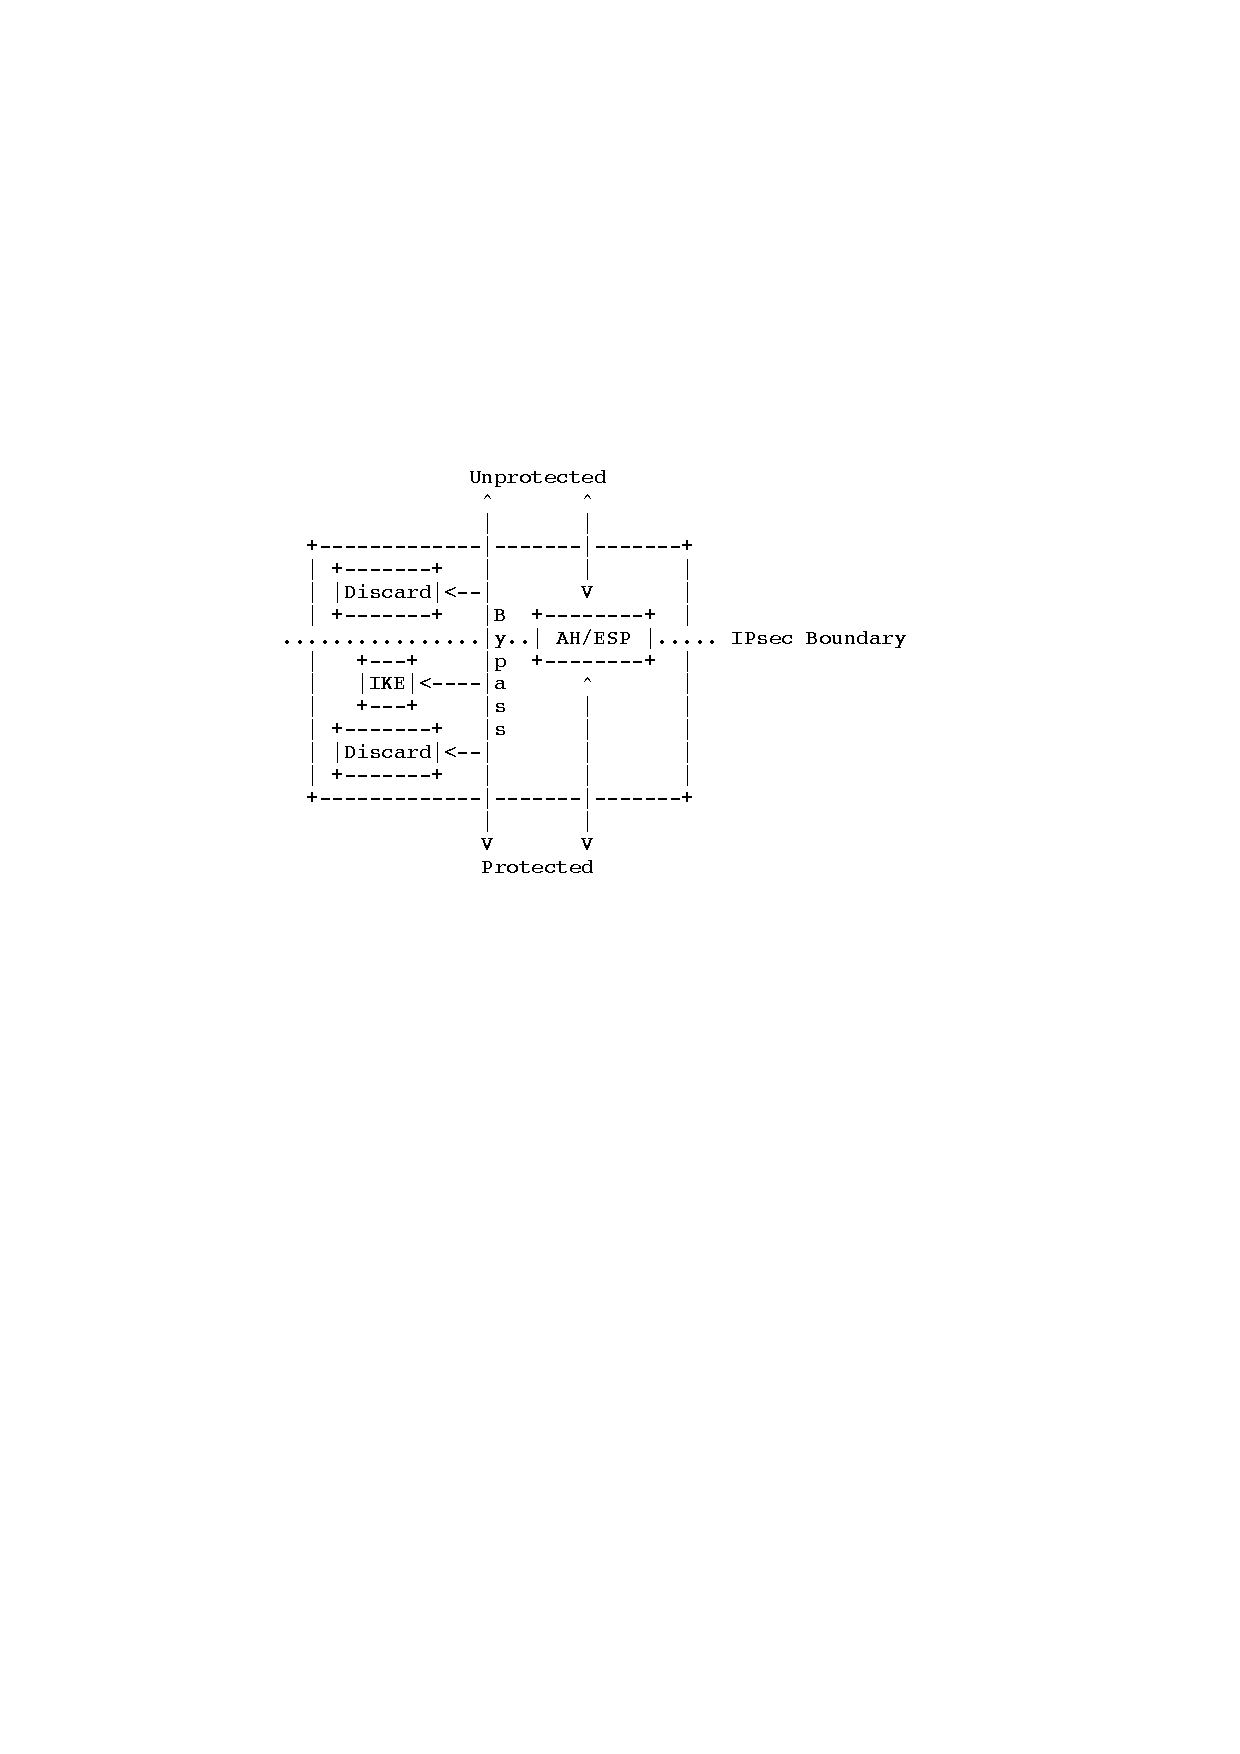
\includegraphics[width=0.9\textwidth]{ipsec-flow}
   \caption{IPsec processing of IP-packets. From \citep[p.8]{rfc4301}.}
   \label{fig:ipsec-flow}
\end{figure}
\label{ipsec_proc}
\paragraph{In the IPsec processing model} IP-packets are said to be passed between from \emph{protected} to \emph{unprotected} interfaces and vice versa. In the usual case, such as above, there are only one of each. The unprotected interface is always the interface connected to the insecure network, while the protected may be either connected to a secure network (the \emph{security gateway} configuration) or be attached to an operating system's IP stack (FIX: Is the last statement ok?). The flow of packets between the protected and unprotected interfaces are determined by policies set by the system administrator which are expressed in terms of network- and transport-layer primitives, i.e. IP addresses, port numbers and transport-layer protocols. The policy can cause a packet to be: thrown away (\emph{DISCARD}); forwarded over the IPsec boundary without any action taken (\emph{BYPASS}; removing or applying cryptographic protection of the packet (\emph{PROTECT}). The later is performed in the module named \emph{AH/ESP} in the fig. no. \ref{fig:ipsec-flow} which we will discuss in length further on (FIX: NO ref to place of disc.?).

\paragraph{A central concept} of the IPsec model is the data structure named the \emph{Security Association} (SA). A Security Association defines a single simplex IP link and the security services it provides to the traffic that it carries. The services can be implemented by one of the two IPsec protocols: \emph{Authentication Header} (AH) and \emph{Encapsulating Security Payload} ESP. Bi-directional (duplex) traffic is enabled by creating a pair of SAs, one for each direction. As the author will show, the SA is used by almost all IPsec components and we will return to it from time to time.

\paragraph{The policies and cryptographic secrets} used in IPsec processing are stored in three databases: the Security Association Database (\emph{SAD}); the Security Policy Database (\emph{SPD}); the Peer Authorization Database (\emph{PAD}). The standard stresses the fact that the implementation of these databases should not be viewed as pre-requisites for a compliant IPsec implementation, but that such a system should exhibit the very same behavior as that of a system whose architecture was implemented in line with the standard's model. In the following paragraphs these databases will be used as constructs to explain the inner workings of IPsec, although, as the reader will learn in the chapter Implementation\ref{chap:Implementation}, the author has actually used these constructs in the final implementation as well. Finally, the system will be explained only in brief as the suite is simply too large for a thorough review in this thesis. The interested reader is advised to read the complete standard document\citep{rfc4301} starting at section 4.4 for an in-depth definition of the SAD, SPD and PAD.


\paragraph{The SPD} stores the policies that controls IPsec processing. It consists of an ordered list, where each entry is composed of a set of \emph{selectors}, \emph{PFP flags} and a \emph{processing action}. 

The \emph{selector} is a data structure that represents a traffic pattern between hosts or networks and serves to distinguish what traffic the policy in question is referring to. The fields are as follows: Local address; Remote address; Next Layer Protocol (e.g. TCP, UDP, ICMP); Local Port (This is dependent upon protocol type, e.g. in the case of an ICMP packet message type and code is listed instead.); Remote Port. Full specifications are found in \citep[Section 4.4.1.1]{rfc4301}.

PFP, or \emph{Populate From Packet} flags, are rules used in conjunction with the instantiation of an SA on the basis of the SPD entry. Instantiation in this context means that the newly created SA's selector (which has a similar purpose to a SPD entry's selector) is completed with information from that of the SPD entry's selector. However, for each of the selector's fields there is a corresponding PFP flag. If that flag is set, that field will be populated with information from the packet that triggered the instantiation. This process will be explained in detail further on as it's a central mechanism.

The processing actions are the very same as described in \ref{ipsec_proc}: \emph{DISCARD}; \emph{BYPASS}; \emph{PROTECT}. The action \emph{PROTECT} differs from the the other actions in the sense that is also includes settings of how to protect the traffic, e.g. using a security gateway (tunneling), DSCP\footnote{Differentiated Services Code Point; QoS control for IPv6} services, various SA settings used in instantiation.


\paragraph{The SAD} stores the IPsec system's \emph{Security Associations} (SAs). The purpose of the database is to store the parameters of the system's SAs, but can be used to store other information as well. RFC 4301 outlines in section 4.4.2.1 fifteen required fields and because of space constraints, this section will only list the ones deemed most important by the author.

Security Parameter Index (SPI): Each SA is identified by a 32-bit value. This value is selected by the receiving end of an SA to be unique. This makes it possible for a system to uniquely associate inbound traffic with an SA using the SPI number as the key. Outbound traffic processing uses the SPI number to construct the IPsec headers.

Sequence Number Counter: Every IPsec system maintains a counter for each SA that is incremented by one for each packet that it carries. This information is used in IPsec packet processing and anti-replay protection (as will be explained below.)

Anti-Replay Window: A counter and a bit-map used for detecting packets that have been replayed by an attacker\footnote{In a replay attack, a packet is intercepted by a man-in-the-middle with the purpose of delaying or repeating it. This can trick the targeted system into revealing secret information e.g. reusing the same keys in a stream cipher.}.

Symmetric encryption information: Encryption algorithm and IPsec protocol type (AH or ESP) used by the SA along with necessary secrets (keys etc) and parameters.

SA Lifetime: A limit at which the SA should be terminated, expressed in either time or the number of bytes transported by the SA.

%each containing the parameters of , each consisting of the following substructures: a \emph{selector}, and an \emph{action}.


\paragraph{The PAD} (section 4.4.3) is controlled by the administrator and used by the security association management protocol along with the SPD to negotiate new SAs. The core purpose of the database is to store 1) the identification tokens of the peers that the system is allowed to communicate with and 2) the authentication mechanism, parameters and data for each aforementioned peer.


% stores the authentication requirements for 5. As SAs can be created both manually by an administrator as well as automatically by a Key Exchange service such as IKE, 

%Security policies are stored in in the \emph{Security Policy Database} (SPD). It consists of several entries, each consisting of the following fields: a \emph{selector} that defines a certain traffic flow; . The selector includes source address range, destination address) by means of \emph{}
% 
%  are said to be members of a communication session for which the same security policies are applied. Such sessions can be   that can be implemented directly in the IP stack of a host or in a router 

\paragraph{IPsec's security model} differs from that of the one commonly used by security protocols operating in the higher layers e.g. TLS and SSH. Instead of using primitives such as user identity or tickets to create secure connections or make policies, IPsec  uses the concept know to IP such as hosts, networks and upper layer protocols such as TCP or UDP.  and .. primitives known to IP; ports, transport layer protocols, networks and host IP-addresses. 

host-to-host
network-to-network
SAD
SPD


\paragraph{Understanding the IP headers} are key to understanding IPsec. The author will therefore quickly review the structure of the IPv6 headers before moving on the explain their relationship to IPsec. Below the readers finds a schematic of the IPv6 header, also called the IPv6 `fixed header' for reasons that soon are to be discussed.

\begin{figure}[here]
   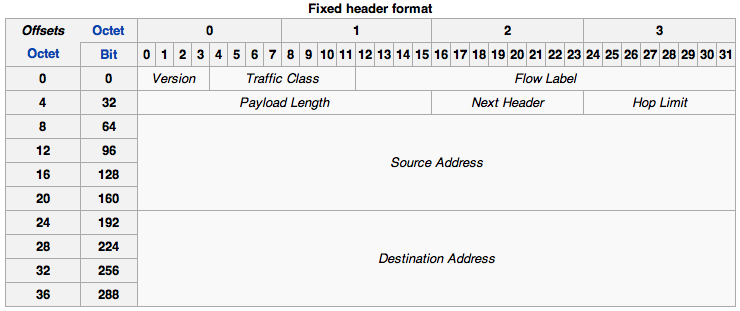
\includegraphics[width=0.9\textwidth]{wiki-ipv6-header}
   \caption{The IPv6 header. Figure from \cite{wiki:ipv6_packet}.}
   \label{fig:ipv6_packet}
\end{figure}

As the author assumes that the reader i acquainted with the general principles of IP networking, the discussion of the above header fields will be brief. \emph{Version} is always six; \emph{Traffic Class} (reminiscent of the IPv4 \emph{TOS} field) and \emph{Flow Label} are for flow and congestion control, which are of no concern to us; \emph{Payload Length} is the length of the payload field, including any so called `extension header' (more on this soon); \emph{Next Header} specifies the packet's transport layer protocol, or the first extension header's type if one is present; \emph{Hop Limit} is equivalent to IPv4's Time-To-Live field which is decremented by each router that it passes, ultimately to be discarded when it reaches zero.

IPv4 placed all of its settings into one big header, many settings which as of today are rarely used, and there was no possibility of extending it for new features. The designers of IPv6 solved this problem in an ingenious way by keeping the fixed header (figure \ref{fig:ipv6_packet}) small and allowing it to be extended by a mechanism called \emph{extension headers}. The extension headers contain any optional information, information which can be intended for the packet's destination host and/or intermediate routers along its path. Although the information is usually supplied by the source host, some headers (such as \emph{Fragment}) can be altered and/or added by routers.

\begin{figure}[here]
   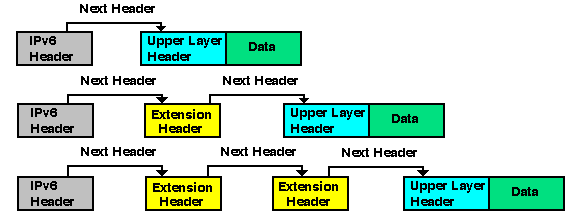
\includegraphics[width=0.9\textwidth]{ipv6-nextheader}
   \caption{Illustration of IPv6's next header scheme. FIX! Not received permission! Source:http://www.zytrax.com/tech/protocols/ipv6.html}
   \label{fig:ipv6_nextheader}
\end{figure}

\begin{figure}[here]
   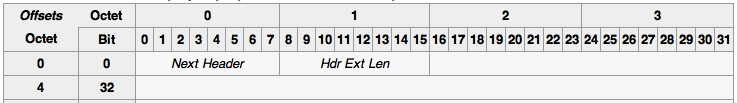
\includegraphics[width=0.9\textwidth]{wiki-ipv6-nextheader}
   \caption{The generic mandatory part of an `extension header'. Figure from \cite{wiki:ipv6_packet}.}
   \label{fig:wiki-ipv6-nextheader}
\end{figure}

The extension header scheme is basically a linked list (figure \ref{fig:wiki-ipv6-nextheader}). The field \emph{Next Header} denotes the type of extension header to come or, if this is the last extension header, the packet's type of transport layer; \emph{Hdr Ext Len} is the length of this extension header in multiples of eight octets, not including the first eight octets. The rest of the next header contains data that is specific to each next header type.

\begin{figure}[h!]
   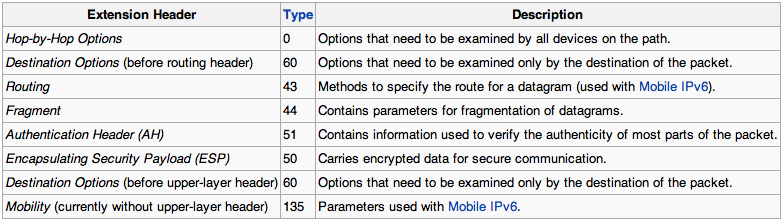
\includegraphics[width=0.9\textwidth]{wiki-ipv6-listofextensionheaders}
   \caption{This list covers a number of common extensions headers `next header'. List from \cite{wiki:ipv6_packet}.}
   \label{fig:wiki-ipv6-nextheader}
\end{figure}


\section{The IPv6 AH extension header}
\begin{figure}[h!]
   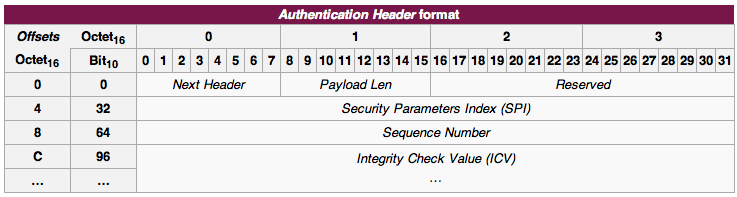
\includegraphics[width=0.9\textwidth]{wiki-ipsec-ah}
   \caption{The AH extension header. From \cite{wiki:ah_header}.}
   \label{fig:wiki-ipsec-ah}
\end{figure}

The AH header guarantees the \emph{data integrity} and the \emph{authentication} (origin) of the IP packet which it is applied to. This is achieved by 

\begin{figure}[h!]
   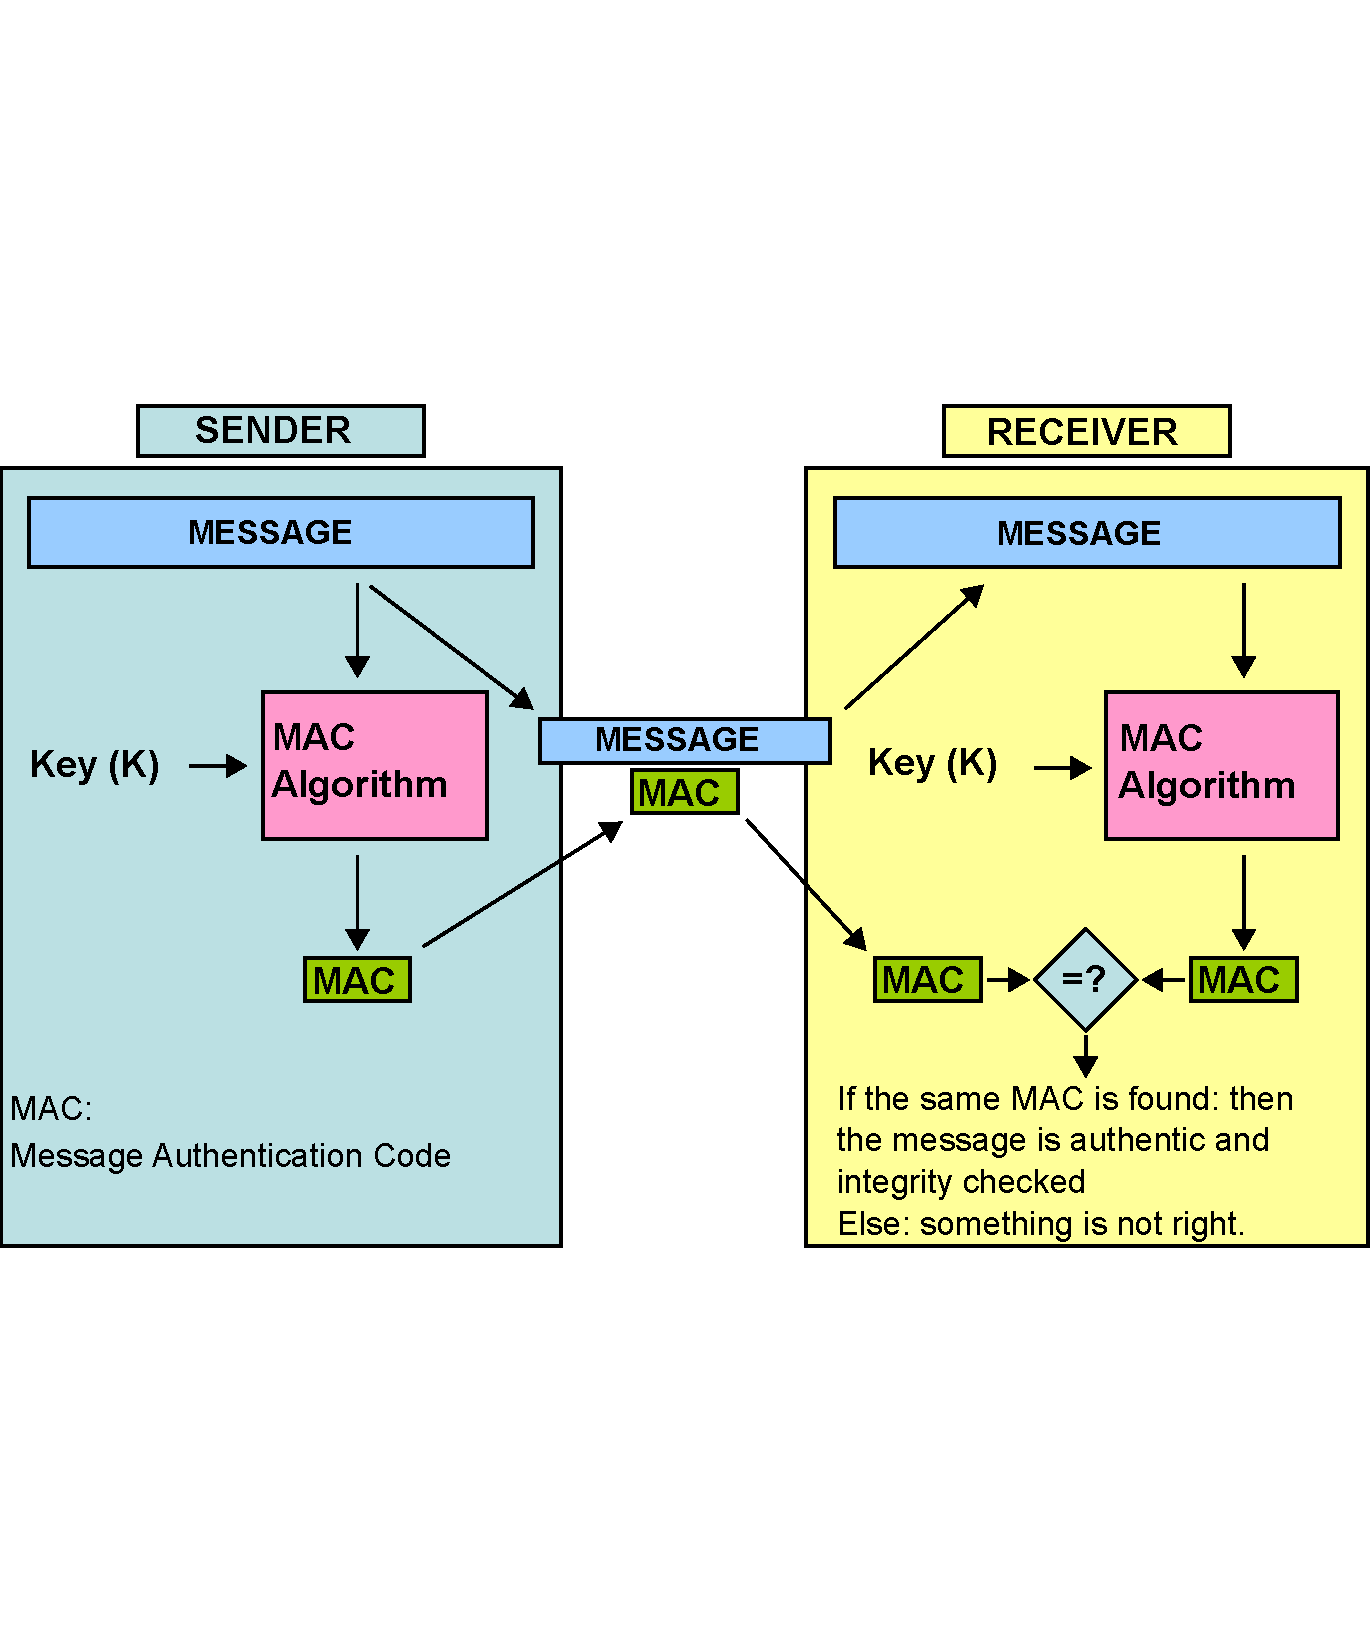
\includegraphics[width=0.9\textwidth, trim=0 205 0 210]{wiki-mac}
   \caption{Message Authentication Code. From \cite{wiki:mac}.}
   \label{fig:wiki-mac}
\end{figure}



HMAC


\section{The IPv6 ESP extension header}


\section{The extension headers ESP and AH}
IPsec makes use of two extension headers, ESP (Encapsulating Security Payload), and AH (Authentication Header). These are used for storing the protected data and products thereof such as checksums and identifying information.

\paragraph{Two of these extension headers are ESP and AH extension headers are dedicated to IPsec}

In order to understand what IPsec does and doesn't do, one has to understand the 

\cite{wiki:ipv6_packet}

 architecture has always been open
* Protects everything from the network level and up (Model)
* Symmetric encryption
* Security associations

\section{Establishing Secure Communication Channels (IKEv2)}
* Handshakes for IPsec
* Establishing security associations
* Asymmetric encryption

\chapter{Design and Implementation} 
Implementing Internet standards in Contiki is often a challenging task. Internet standards are written with the presumption of hosts with vastly more capable hardware on the host's part. This requires the engineer to simplify parts of the standard, make generalizations, and omit parts altogether. This might be difficult as it requires good knowledge of the standard in question as well as the behavior of other implementations. The synthesis of this knowledge allows her to save hardware resources by making shortcuts in her implementation, shortcuts which might very well violate the standard document, but still exhibit a behavior which allows communication with the rest of the Internet. This a good example of the very practical, experimental, approach that is typical of Contiki's development culture.

\section{Development process}
The original goal of this thesis was to develop a working IKEv2 implementation on top of of an existing IPsec implementation already developed for Contiki. Therefore the literature review started with the RFCs\footnote{Described in so the so called RFC (Request for Comments) publication managed by the IETF and the Internet Society} covering that standard, continuing with other documents as the author's understanding of the field grew. 

The author found the body of standard documents to be large, complex and described many features. It was unclear what effects a removal or alteration of a behavior could have on the implementation. Therefore the following principle was decided upon:

\begin{quote}
\emph{The guiding design principle of the implementation} is that is must be a subset of the standard and follow the described architecture as close as possible. Any deviation from this requires a thorough analysis of the security implications or the implementation will lose its greatest benefit - the security properties brought by the thoroughly vetted IPsec standard.
\end{quote}

Obviously, a thorough investigation and rework of the standards' internals would have the possibility of resulting in a more efficient implementation, but such an endeavor would require an effort that certainly would be outside the bounds of this work. 

Simultaneously, the author worked with Contiki's source code and documentation in order to figure out how to integrate IKEv2 and the IPsec system into Contiki, a feat easier said than done as Contiki is quite different from the typical multi-user multi-tasking operating system. Implementation then proceeded in a top-down fashion where the data structures were written first, APIs secondly and then finally the actual algorithms.

Contiki targets\footnote{A compiler is said to be \emph{targetting} a certain CPU's instruction set in the sense that it is configured to produce compatible binaries.} many different platforms, and two of them is Windows and Linux, i.e. the platform that the compiler is running on. This is called the \emph{native} target and is particular in the sense that Contiki (which is running as an ordinary process in the host's operating system) has access to the wast resources of the personal computer. Needless to say, this greatly facilitates debugging and was therefore used as the predominant build target during the development process. Peripherals such as sensors are emulated and network communication is achieved using a faked serial interface over a tunnel FIX:Look this up. 

\paragraph{During final development} the target was changed from \emph{native} to \emph{msp430} (a CPU commonly used in IoT platforms due to its energy efficiency) as the focus turned from functionality to memory and speed improvements. Benchmarking and tuning has to be performed on the correct platform as libraries, the platform's instruction set, and compiler optimization possibilities are target specific. Instead of using actual hardware\footnote{Using real hardware for testing purposes turned out to be a large problem as no readily available platform had the required memory capacity to store the binaries.} Contiki was executed on emulated hardware using Contiki's popular simulation environment - Cooja\cite{osterlind06crosslevel}. Apart from providing emulation, Cooja features a complete experimental sandbox which will be further described in the chapter Evaluation.


% As the author only had a rudimentary knowledge (roughly comparable as that of system administrator) of IPsec / IKEv2, he decided to that the safest way.

\section{IPsec}
We implement IPsec by inserting hooks into the uIP-stack.

IPsec and IKE communicates through the databases SPD and SAD. The PAD doesn't need to be a database.

The IPsec subsystem is implemented inside the uIP6 stack.

[BIG image outlining what information is passed between the IP-stack, the IPsec processing subsystem, IKEv2 and the databases (SPD, SAD)]


\section{IKEv2}
The IKEv2 service is implemented as a Contiki Process. Each session is modelled as a mealy state machine [img].

The machine is built to be extended. The following is implemented as of now:


\chapter{Evaluation}

\section{Memory requirements}
Maximum stack and heap requirements
Per SA requirement

\section{Latency}
* IKE handshake: Energy and time. Total setup time.
* IPsec packet: Energy required for receiving, energy required for transmitting. Roundtrip times.

\chapter{Improvements}


\bibliography{refs,rfc}
\bibliographystyle{plain}

\end{document}

% SLUT!














\section{IoT}

SICS\footnote{Swedish Institute of Computer Science} have been conducting research the field of IoT for over a decade. The purpose is to explore, and try to solve, the problems in the software stack. One of these areas is end-to-end security between a host in the IoT network and one on the Internet.

 This has resulted in the very small event driven operating system Contiki. 

Why we want IoT.
In order to bring IoT out of the lab and into the society it needs to be secure. A pair of hosts in the network must be able to authenticate each other and protect their communication from privy eyes by means of encryption. The solution concerned also needs to be standards-compliant with the rest of the Internet.

This suggests that TLS or IPsec may be suitable.

TLS secures a TCP connection. IPsec secures everything from the network layer and up. The purpose of this work is to implement IPsec and IKEv2 

The topic of this work is to implement IPsec and IKEv2 with the purpose of investigating the following:


\subsection{The Contiki OS}%\footnote{Internet of Things}}
Contiki is an event based operating system...

\subsection{IPsec}
IPsec is an IETF\footnote{Internet Engineering Task Force} standard defined in RFC ...

\subsection{TLS}
TLS is a ...

\section{Scope}

The purpose of this thesis is to explore the IPsec venue; is it a feasible solution?

\subsection{Motivation}

The goal of the thesis is to write an implementation of IPsec and IKEv2 in order to prove that the following is possible:
* Low power, resource constrained hardware can utilize ``heavy'' Internet-standards and asymmetric encryption
* The implementation should be able to communicate with a wide range of systems

From this, the following should be required in order to form a valid proof-of-concept:
* The implementation should be polite towards other hosts. It should be able to handle a wide range of situations.
* Where time does not allow for a full implementation of a certain functionality, it should be clear that the implementation can be extended without significant rewrites of other parts.

The original scope was the implementation of the IKEv2 service as described in RFC 5996 [...] for the Contiki OS. After a more thourough investigation this was found not to be feasible.


\chapter{Design}
The purpose of the
The original design goals requirements of the implementation were
1) It should implement a subset of IPsec and IKEv2 where feasible, or 
2) 
chose
choose
chosen

\section{Constraints}
Memory, processing, energy...


\chapter{Implementation}
GCC, utveckling på PC-hårdvara
Hanterverket
(kort avsnitt)


\chapter{Evaluation}
Evaluation of the impl. in relation to the design goals


\section{Performance and requirements}
Processing and memory requirements

\section{Design evaluation}
Implications of design choices

\section{Recommendation}
cite:Problem Areas for the IP Security Protocols



\end{document}
